% !TeX program = xelatex
% EverOS v1: Physically Isolated Memory API for Multi-Agent Systems
% Compile: latexmk -xelatex everos-techreport.tex
% arXiv tech report — companion to "When Agents Remember, They Stop Building"

\documentclass[11pt, a4paper]{article}

% ═══════════════════════════════════════════════════════════
% PACKAGES
% ═══════════════════════════════════════════════════════════
\usepackage[top=25mm, bottom=28mm, left=25mm, right=25mm]{geometry}
\usepackage{fontspec}
\setmainfont{texgyrepagella-regular.otf}[
  BoldFont = texgyrepagella-bold.otf,
  ItalicFont = texgyrepagella-italic.otf,
  BoldItalicFont = texgyrepagella-bolditalic.otf,
]
\setsansfont{texgyreheros-regular.otf}[
  BoldFont = texgyreheros-bold.otf,
  ItalicFont = texgyreheros-italic.otf,
  Scale = 0.95,
]
\setmonofont{texgyrecursor-regular.otf}[
  BoldFont = texgyrecursor-bold.otf,
  Scale = 0.85,
]
\usepackage[protrusion=true]{microtype}
\usepackage{setspace}
\setstretch{1.15}
\setlength{\parindent}{0pt}
\setlength{\parskip}{0.5em}

\usepackage[dvipsnames,table]{xcolor}
\definecolor{deep}{RGB}{53,88,76}
\definecolor{accent}{RGB}{240,238,155}
\definecolor{faded}{RGB}{127,136,130}
\definecolor{subtle}{RGB}{238,235,225}
\definecolor{errcoral}{RGB}{255,107,128}
\definecolor{obsblue}{RGB}{70,130,180}
\definecolor{rungreen}{RGB}{86,190,120}
\definecolor{voidgray}{RGB}{160,160,160}
\definecolor{ctrlpurp}{RGB}{150,110,180}

\usepackage{titlesec}
\titleformat{\section}{\sffamily\Large\bfseries\color{deep}}{\thesection}{0.7em}{}
\titleformat{\subsection}{\sffamily\large\color{deep}}{\thesubsection}{0.6em}{}
\titleformat{\subsubsection}{\sffamily\normalsize\itshape\color{faded}}{\thesubsubsection}{0.5em}{}

\usepackage{tikz}
\usetikzlibrary{arrows.meta, positioning, fit, calc, backgrounds, shapes.geometric}
\usepackage{listings}
\usepackage{tabularray}
\usepackage{adjustbox}
\usepackage{enumitem}
\usepackage{float}
\usepackage{amsmath}
\usepackage{amssymb}
\usepackage{hyperref}
\hypersetup{colorlinks=true, linkcolor=deep, citecolor=deep, urlcolor=deep!70}

\lstdefinelanguage{TypeScript}{
  keywords={async, await, function, const, let, return, export, class, new, import, from, interface, type, extends, implements, if, else, throw, try, catch, typeof, public, private, readonly, Promise, string, number, boolean, unknown, void, true, false, null, undefined},
  morecomment=[l]{//},
  morecomment=[s]{/*}{*/},
  morestring=[b]',
  morestring=[b]",
  morestring=[b]`,
  sensitive=true,
}
\lstset{
  language=TypeScript,
  basicstyle=\ttfamily\small,
  keywordstyle=\bfseries\color{deep},
  commentstyle=\itshape\color{faded},
  stringstyle=\color{deep!60},
  backgroundcolor=\color{subtle!50},
  frame=single,
  rulecolor=\color{deep!20},
  framesep=6pt,
  xleftmargin=6pt,
  xrightmargin=6pt,
  breaklines=true,
  showstringspaces=false,
  tabsize=2,
  captionpos=b,
  aboveskip=8pt,
  belowskip=8pt,
}

% ═══════════════════════════════════════════════════════════
% TITLE
% ═══════════════════════════════════════════════════════════
\title{%
  \sffamily\bfseries
  EverOS v1: Physically Isolated Memory API\\
  for Multi-Agent Systems%
}
\author{%
  Hengyuan Zhu\\
  {\small University of South Carolina}\\
  {\small\texttt{fearvox1015@gmail.com}}
}
\date{April 2026}

\begin{document}
\maketitle

% ═══════════════════════════════════════════════════════════
% ABSTRACT
% ═══════════════════════════════════════════════════════════
\begin{abstract}
Multi-agent AI systems require persistent memory, yet existing memory frameworks (MemGPT, Reflexion, LangGraph) provide only logical partitioning within a shared namespace---insufficient for controlled experiments and secure production deployments. We present \textbf{EverOS v1}, a RESTful memory API that enforces \textbf{physical isolation} at the API key level: each key maps to an independent memory space with zero cross-namespace access by construction. The API exposes 6 modules (Memories, Groups, Senders, Tasks, Storage, Settings) with three-tier memory scoping (Personal, Group, Agent) and sender identity tracking for full audit trails.

We describe three contributions: (1) the 4-key experimental design that enables $2 \times 2$ factorial studies of memory effects (Observer, Runner, Void, Control keys), used in a companion study~[1] that found memory explains 91.7\% of behavioral variance ($\eta^2 = .917$); (2) sender identity tracking that made recursive memory contamination traceable; and (3) convenience patterns (\texttt{createObserverClient}, \texttt{createRunnerClient}, \texttt{createVoidClient}) that reduce experimental configuration errors. We validate these designs through 13 benchmark rounds and a 6-agent production deployment with Ebbinghaus-based memory decay. The client library is 394 lines of dependency-free TypeScript.
\end{abstract}

% ═══════════════════════════════════════════════════════════
% 1. INTRODUCTION
% ═══════════════════════════════════════════════════════════
\section{Introduction}

Persistent memory is becoming a core component of production AI agent systems. Tools such as Claude Code, GitHub Copilot Workspace, and Cursor now maintain cross-session state that influences agent decisions in subsequent interactions. A companion study~[1] demonstrates that persistent memory explains 91.7\% of variance in agent engineering strategy---agents with memory redefine ``build from scratch'' as ``maintain and optimize existing systems.''

Yet the memory infrastructure underlying such experiments faces a fundamental design choice: \textbf{logical isolation} vs.\ \textbf{physical isolation}. Logical isolation partitions memories within a single namespace via access control rules; physical isolation assigns each participant an independent namespace with no shared state.

Existing systems choose logical isolation:
\begin{itemize}[nosep]
  \item \textbf{MemGPT}~[2]: Single-user virtual memory paging---no multi-agent namespace separation.
  \item \textbf{Reflexion}~[3]: Episodic verbal feedback stored per-agent but with no persistent backing store or cross-session isolation.
  \item \textbf{LangGraph}: Shared state graph with node-level access---logical partitioning within one execution graph.
\end{itemize}

Logical isolation is sufficient for cooperative systems but inadequate for two critical scenarios:

\textbf{Controlled experiments.} Studying how memory affects agent behavior requires \emph{provable non-contamination} between experimental conditions. Logical partitions can leak through misconfigured access control, shared embedding indices, or API-level side channels. Physical isolation eliminates these vectors by construction.

\textbf{Adversarial multi-agent settings.} Production deployments with heterogeneous agents (different models, runtimes, trust levels) require that a compromised agent cannot access another agent's memory even with a valid authentication token.

This report describes EverOS v1, a memory API designed for physical isolation. We focus on three aspects: API surface design (\S2), the physical isolation model and its experimental applications (\S3), and sender identity tracking for audit trails (\S4). We validate through benchmark experiments (\S5) and a production deployment (\S6).

% ═══════════════════════════════════════════════════════════
% 2. API DESIGN
% ═══════════════════════════════════════════════════════════
\section{API Design}

EverOS v1 exposes a RESTful API at \texttt{https://api.evermind.ai/api/v1} with Bearer token authentication. The TypeScript client organizes the API into 6 modules:

\subsection{Module Architecture}

\begin{adjustbox}{max width=\linewidth}
\begin{tblr}{
  colspec = {l l X[l] l},
  row{1} = {font=\sffamily\bfseries\small, bg=deep, fg=white},
  hlines = {deep!20}, rowsep = 6pt, colsep = 8pt,
}
Module & Methods & Description & Endpoint Prefix \\
Memories & 10 & Add, search, get, delete, flush (3 scopes) & \texttt{/memories/} \\
Groups & 3 & Create (upsert), get, update & \texttt{/groups/} \\
Senders & 3 & Create, get, update & \texttt{/senders/} \\
Tasks & 1 & Background task status polling & \texttt{/tasks/} \\
Storage & 1 & Pre-signed S3 upload URLs & \texttt{/storage/} \\
Settings & 2 & Get, update (full replace via PUT) & \texttt{/settings/} \\
\end{tblr}
\end{adjustbox}

The client is instantiated with a single API key that determines the physical memory space:

\begin{lstlisting}[caption={Client initialization (from \texttt{everos.ts}:319--332)}]
const client = new EverOSClient(OBSERVER_KEY)
// All subsequent calls operate within this key's memory space
// Modules are accessed as properties:
client.memories   // MemoriesModule (10 methods)
client.groups     // GroupsModule (3 methods)
client.senders    // SendersModule (3 methods)
client.tasks      // TasksModule (1 method)
client.storage    // StorageModule (1 method)
client.settings   // SettingsModule (2 methods)
\end{lstlisting}

\subsection{Three-Tier Memory Scoping}

Within a single memory space (determined by the API key), memories are further scoped along three dimensions:

\begin{lstlisting}[caption={Memory scoping API (from \texttt{everos.ts}:124--163)}]
// Personal scope: user-specific memories
await client.memories.addPersonal(userId, messages, {
  metadata: { source: 'benchmark' },
  infer: true  // server-side inference extraction
})

// Group scope: shared within a named group
await client.memories.addGroup(groupId, messages)

// Agent scope: private to a specific agent identity
await client.memories.addAgent(agentId, messages)
\end{lstlisting}

All three scoping methods call the same REST endpoint (\texttt{POST /memories/}) with different scope identifiers (\texttt{user\_id}, \texttt{group\_id}, \texttt{agent\_id}). The server enforces that memories written under one scope are not retrievable under another.

\subsection{Search: Hybrid and Agentic Modes}

The API supports two search modes through the same endpoint (\texttt{POST /memories/search/}):

\begin{lstlisting}[caption={Search modes (from \texttt{everos.ts}:166--185)}]
// Hybrid search: vector similarity + keyword matching
const results = await client.memories.search({
  query: 'parallel deployment strategy',
  user_id: userId,
  top_k: 10,
  filters: { source: 'benchmark' }
})

// Agentic search: context-aware retrieval
const agenticResults = await client.memories.agenticSearch({
  query: 'parallel deployment strategy',
  user_id: userId,
  // search_type: 'agentic' is set internally
})
\end{lstlisting}

Hybrid search returns scored results ranked by embedding similarity; agentic search applies additional contextual reasoning to return memories most relevant to the agent's current task.

\subsection{Flush and Knowledge Extraction}

Flush operations trigger server-side Cases \& Skills extraction before clearing memories:

\begin{lstlisting}[caption={Flush operations (from \texttt{everos.ts}:199--220)}]
// Flush personal memories (triggers extraction pipeline)
await client.memories.flushPersonal(userId)
// Flush group memories
await client.memories.flushGroup(groupId)
// Flush agent memories
await client.memories.flushAgent(agentId)
\end{lstlisting}

These operations are critical for benchmark hygiene: flushing the Void space between runs ensures clean-room conditions while preserving extracted knowledge patterns.

% ═══════════════════════════════════════════════════════════
% 3. PHYSICAL ISOLATION MODEL
% ═══════════════════════════════════════════════════════════
\section{Physical Isolation Model}

\subsection{Key-Level Isolation}

The fundamental design principle: \textbf{each API key maps to an independent memory space}. Two clients instantiated with different keys share nothing---no memories, no groups, no senders, no settings. This is enforced server-side; the client library does not implement any isolation logic.

\begin{figure}[H]
\centering
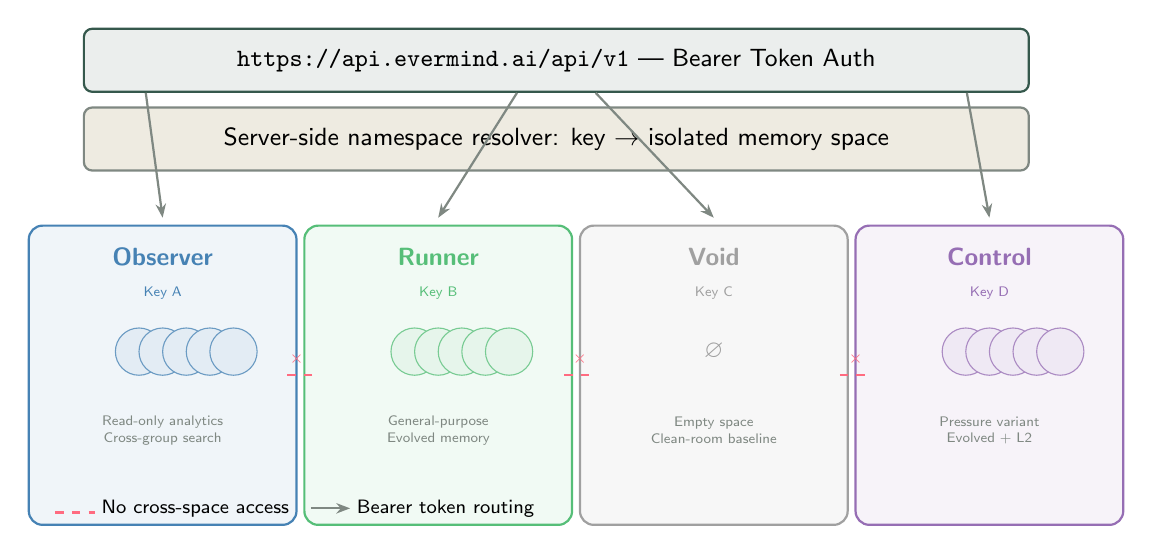
\begin{tikzpicture}[
  keybox/.style={draw=#1, fill=#1!8, rounded corners=5pt, minimum width=3.4cm, minimum height=3.8cm, thick, align=center},
  memcircle/.style={circle, draw=#1!80, fill=#1!15, minimum size=0.6cm, inner sep=0pt, font=\sffamily\tiny},
  keylabel/.style={font=\sffamily\bfseries\small, color=#1},
  api/.style={draw=deep, fill=deep!10, rounded corners=3pt, minimum width=12cm, minimum height=0.8cm, font=\sffamily\small, thick},
  server/.style={draw=faded, fill=subtle, rounded corners=3pt, minimum width=12cm, minimum height=0.8cm, font=\sffamily\small, thick},
  arr/.style={-{Stealth[length=5pt]}, thick, color=faded},
  noarr/.style={thick, color=errcoral, dashed},
]
  % API layer
  \node[api] (api) at (0, 4.5) {\texttt{https://api.evermind.ai/api/v1} --- Bearer Token Auth};
  \node[server] (srv) at (0, 3.5) {Server-side namespace resolver: key $\to$ isolated memory space};

  % Four key boxes
  \node[keybox=obsblue] (obs) at (-5, 0.5) {};
  \node[keylabel=obsblue] at (-5, 2.0) {Observer};
  \node[font=\sffamily\tiny\color{obsblue}] at (-5, 1.55) {Key A};
  \foreach \i in {1,...,5} {
    \node[memcircle=obsblue] at (-5.6+\i*0.3, 0.8) {};
  }
  \node[font=\sffamily\tiny\color{faded}, text width=2.8cm, align=center] at (-5, -0.2) {Read-only analytics\\Cross-group search};

  \node[keybox=rungreen] (run) at (-1.5, 0.5) {};
  \node[keylabel=rungreen] at (-1.5, 2.0) {Runner};
  \node[font=\sffamily\tiny\color{rungreen}] at (-1.5, 1.55) {Key B};
  \foreach \i in {1,...,5} {
    \node[memcircle=rungreen] at (-2.1+\i*0.3, 0.8) {};
  }
  \node[font=\sffamily\tiny\color{faded}, text width=2.8cm, align=center] at (-1.5, -0.2) {General-purpose\\Evolved memory};

  \node[keybox=voidgray] (vd) at (2, 0.5) {};
  \node[keylabel=voidgray] at (2, 2.0) {Void};
  \node[font=\sffamily\tiny\color{voidgray}] at (2, 1.55) {Key C};
  \node[font=\sffamily\small\color{voidgray}] at (2, 0.8) {$\varnothing$};
  \node[font=\sffamily\tiny\color{faded}, text width=2.8cm, align=center] at (2, -0.2) {Empty space\\Clean-room baseline};

  \node[keybox=ctrlpurp] (ctrl) at (5.5, 0.5) {};
  \node[keylabel=ctrlpurp] at (5.5, 2.0) {Control};
  \node[font=\sffamily\tiny\color{ctrlpurp}] at (5.5, 1.55) {Key D};
  \foreach \i in {1,...,5} {
    \node[memcircle=ctrlpurp] at (4.9+\i*0.3, 0.8) {};
  }
  \node[font=\sffamily\tiny\color{faded}, text width=2.8cm, align=center] at (5.5, -0.2) {Pressure variant\\Evolved + L2};

  % Arrows from API to keys
  \draw[arr] (api.south west) ++(0.8,0) -- (-5, 2.5);
  \draw[arr] (api.south) ++(-0.5,0) -- (-1.5, 2.5);
  \draw[arr] (api.south) ++(0.5,0) -- (2, 2.5);
  \draw[arr] (api.south east) ++(-0.8,0) -- (5.5, 2.5);

  % No-cross arrows
  \draw[noarr] (-3.1, 0.5) -- (-3.5, 0.5) node[midway, above, font=\sffamily\tiny\color{errcoral}] {$\times$};
  \draw[noarr] (0.1, 0.5) -- (0.5, 0.5) node[midway, above, font=\sffamily\tiny\color{errcoral}] {$\times$};
  \draw[noarr] (3.6, 0.5) -- (4.0, 0.5) node[midway, above, font=\sffamily\tiny\color{errcoral}] {$\times$};

  % Legend
  \node[font=\sffamily\scriptsize, anchor=west] at (-6.5, -1.2) {
    \begin{tabular}{@{}c@{\;}l@{\quad}c@{\;}l@{}}
    \tikz\draw[thick, color=errcoral, dashed] (0,0) -- (0.5,0); & No cross-space access &
    \tikz\draw[arr] (0,0) -- (0.5,0); & Bearer token routing \\
    \end{tabular}
  };
\end{tikzpicture}
\caption{4-key physical isolation architecture. Each API key routes to an independent memory space. Dashed red lines indicate zero cross-namespace access, enforced server-side. This design directly enables the $2 \times 2$ factorial experiment in~[1].}
\label{fig:isolation}
\end{figure}

\subsection{4-Key Experimental Design}

The physical isolation model directly enables factorial experiments by mapping each experimental condition to an independent key:

\begin{adjustbox}{max width=\linewidth}
\begin{tblr}{
  colspec = {l l l l X[l]},
  row{1} = {font=\sffamily\bfseries\small, bg=deep, fg=white},
  row{2} = {bg=obsblue!8}, row{3} = {bg=rungreen!8}, row{4} = {bg=voidgray!8}, row{5} = {bg=ctrlpurp!8},
  hlines = {deep!20}, rowsep = 6pt, colsep = 8pt,
}
Key & Role & Memory State & Pressure & Factorial Cell \\
A (Observer) & Analytics & Read-only cross-group & --- & Observer (not a cell) \\
B (Runner) & Experiment & Evolved (persistent) & L0 & Memory+, Pressure$-$ \\
C (Void) & Baseline & Empty (clean-room) & L0 & Memory$-$, Pressure$-$ \\
D (Control) & Variant & Evolved (persistent) & L2 & Memory+, Pressure+ \\
\end{tblr}
\end{adjustbox}

The companion study~[1] added a fifth condition (Void + L2) using a separate key for the full $2 \times 2$ matrix ($N=11$). The ANOVA result---memory $\eta^2 = .917$, pressure $p = .072$---is directly attributable to the guarantee that Runner B's memories never leaked into Void C's space, and vice versa.

\subsection{Why Physical over Logical Isolation}

\begin{adjustbox}{max width=\linewidth}
\begin{tblr}{
  colspec = {l X[l] X[l]},
  row{1} = {font=\sffamily\bfseries\small, bg=deep, fg=white},
  hlines = {deep!20}, rowsep = 6pt, colsep = 8pt,
}
Dimension & Logical Isolation & Physical Isolation (EverOS) \\
Contamination vector & ACL misconfiguration, shared indices & None by construction \\
Experimental validity & Requires verification of partition integrity & Guaranteed by architecture \\
Cross-condition leakage & Possible via embedding similarity search & Impossible (separate vector stores) \\
Compromise blast radius & One token exposes entire namespace & One token exposes one key's space \\
Operational complexity & Complex ACL rules, audit needed & Simple: one key per condition \\
\end{tblr}
\end{adjustbox}

% ═══════════════════════════════════════════════════════════
% 4. SENDER IDENTITY TRACKING
% ═══════════════════════════════════════════════════════════
\section{Sender Identity Tracking}

\subsection{The Audit Problem}

In multi-agent systems, memories are written by multiple sources: human operators, AI agents of different models, automated pipelines, and observation systems. Without sender identity, a critical question becomes unanswerable: \textbf{who wrote what to which memory space?}

This question is not merely administrative. The companion study~[1, \S6] documented recursive contamination where Runner B wrote experimental knowledge back into memory, deepening contamination for future runners. Tracing this contamination loop required knowing the write origin of each memory entry.

\subsection{Sender API}

\begin{lstlisting}[caption={Sender identity management (from \texttt{everos.ts}:247--258)}]
// Register a sender identity
const sender = await client.senders.create({
  name: 'benchmark-harness',
  metadata: { version: '2.0', runId: 'R011-B' }
})

// Retrieve sender for audit
const info = await client.senders.get(sender.data.sender_id)

// Update sender metadata (e.g., after run completion)
await client.senders.update(sender.data.sender_id, {
  metadata: { ...info.data.metadata, completed: true }
})
\end{lstlisting}

\subsection{Audit Chain in the Panopticon}

The production deployment~[1, \S6.2] revealed a Panopticon memory topology: the Observer (using Key~A) can search across all memory groups via cross-group search, while each agent reads only its own group. Sender identity makes this topology auditable:

\begin{enumerate}[nosep]
  \item Observer queries all memories across groups
  \item Each memory entry carries a \texttt{sender\_id}
  \item The audit trail answers: Agent-$\alpha$ wrote memory $M_1$ at $T_1$; Runner B wrote $M_2$ at $T_2$
  \item Contamination loops (Runner $\to$ memory $\to$ future Runner) become traceable
\end{enumerate}

This is the foundation for detecting memory injection attacks: if a memory's sender identity does not match expected writers, it signals unauthorized access.

% ═══════════════════════════════════════════════════════════
% 5. CONVENIENCE PATTERNS
% ═══════════════════════════════════════════════════════════
\section{Convenience Patterns and Benchmark Integration}

\subsection{Factory Functions}

To reduce experimental configuration errors, the client library provides pre-configured factory functions:

\begin{lstlisting}[caption={Factory functions (from \texttt{everos.ts}:381--393)}]
// Observer key: read-only analytics space
function createObserverClient(): EverOSClient {
  return new EverOSClient(
    process.env.EVERMEM_OBS_KEY ?? OBSERVER_KEY
  )
}

// Runner key: general-purpose evolved space
function createRunnerClient(): EverOSClient {
  return new EverOSClient(
    process.env.EVERMEM_RNR_KEY ?? RUNNER_KEY
  )
}

// Void key: empty/disposable clean-room space
function createVoidClient(): EverOSClient {
  return new EverOSClient(
    process.env.EVERMEM_VOID_KEY ?? VOID_KEY
  )
}
\end{lstlisting}

Each factory resolves its key from environment variables with a hardcoded fallback. This two-layer resolution enables: (1) local development with default keys, (2) CI/CD with injected secrets, and (3) benchmark harness override via \texttt{isolate.sh} environment variable injection.

\subsection{Harness Integration}

The benchmark harness (\texttt{harness.ts}) uses the EverOS client at two critical points:

\textbf{Pre-run memory classification.} Before each benchmark round, a classifier (\texttt{classify-memory.ts}) audits the memory space and categorizes files as ALLOW (9 safe files), BLOCK (9 files containing experimental knowledge), or GRAY (4 ambiguous files). This classification uses the \texttt{memories.search()} API to inspect the current memory state.

\textbf{Pre/post snapshot differencing.} The harness captures test file snapshots before and after the benchmark subprocess runs, then uses \texttt{diffSnapshots()} to count only genuinely new tests. For full-memory conditions, a pre-run \texttt{bun test} establishes the baseline count, and the harness reports the delta.

\begin{lstlisting}[caption={Harness memory state selection (conceptual, from \texttt{harness.ts}:72--88)}]
// Workspace setup based on memory condition
const workspace = await setupWorkspace(config, logger)
// config.memory determines which key to inject:
//   'full'  -> EVERMEM_RNR_KEY (Runner space, evolved)
//   'void'  -> EVERMEM_VOID_KEY (Void space, clean-room)
//   'none'  -> No EverMem env var (no memory system)
const env = buildEnv(provider, config, workspace)
\end{lstlisting}

% ═══════════════════════════════════════════════════════════
% 6. PRODUCTION DEPLOYMENT
% ═══════════════════════════════════════════════════════════
\section{Production Deployment: 6-Agent Case Study}

\subsection{Three-Layer Memory Architecture}

A 6-agent production deployment (4 Claude Code + 2 Codex CLI agents) validated the API in a collaborative business intelligence setting. The deployment organized memories into three layers:

\begin{adjustbox}{max width=\linewidth}
\begin{tblr}{
  colspec = {l l X[l] l},
  row{1} = {font=\sffamily\bfseries\small, bg=deep, fg=white},
  hlines = {deep!20}, rowsep = 6pt, colsep = 8pt,
}
Layer & Scope & Content & Access \\
Public & \texttt{group\_id} (shared) & Client profiles, industry data, dialogue logs & All agents \\
Restricted & \texttt{group\_id} (limited) & Relationship maps, risk assessments, evolution logs & Admin + Observer \\
Sovereign & \texttt{agent\_id} (per-agent) & Agent-specific strategies, self-assessments & Owner agent only \\
\end{tblr}
\end{adjustbox}

\subsection{Ebbinghaus Decay Integration}

The deployment integrated an Ebbinghaus-based memory decay model with difficulty-graded retention rates:
\begin{itemize}[nosep]
  \item \textbf{Easy} memories (routine data): 24-hour half-life ($R(t) = e^{-t/24}$)
  \item \textbf{Medium} memories (analytical insights): 72-hour half-life
  \item \textbf{Hard} memories (strategic decisions): 168-hour half-life (7 days)
\end{itemize}

Memories below a 30\% retention threshold are archived on the next sweep via \texttt{memories.delete()}, while extracted knowledge patterns are preserved through the flush pipeline.

\subsection{Emergent Panopticon Topology}

The most significant production finding was an emergent Panopticon memory topology. Each Claude Code agent runs in a unique CWD (\texttt{\textasciitilde/.sigma/agents/\{uuid\}/}), and EverMem's group isolation algorithm assigns CWD-based group IDs. This produces:

\begin{itemize}[nosep]
  \item \textbf{Observer $\to$ all agents}: Cross-group search via Observer key reveals all memories (unidirectional)
  \item \textbf{Agent $\to$ self}: Each agent reads only its own group (island)
  \item \textbf{Agent $\to$ other agents}: Completely invisible (mutual isolation)
  \item \textbf{Codex CLI agents}: No EverMem hook, escape observation entirely (0 memories)
\end{itemize}

This topology was not designed---it is a byproduct of the CWD-based grouping algorithm intersecting with the physical isolation model. The Observer's cross-group search capability (available because the Observer key's memory space indexes all groups it has been granted access to) creates an asymmetric surveillance structure at $O(1)$ monitoring cost.

\subsection{Admin-Gate Write Protocol}

To prevent uncontrolled memory accumulation, the deployment enforces an Admin-gate protocol: all writes to the \texttt{restricted/} layer must be approved by the Admin agent before committing via \texttt{memories.addGroup()}. This mirrors the benchmark's memory classification step but applied to production content.

% ═══════════════════════════════════════════════════════════
% 7. LESSONS LEARNED
% ═══════════════════════════════════════════════════════════
\section{Lessons Learned}

\textbf{4-key design enables factorial experiments.} Physical isolation is not just a security feature---it is a \emph{methodological enabler}. Without it, the $2 \times 2$ factorial design in~[1] would require extensive verification that no memory leakage occurred between conditions. With physical isolation, non-contamination is guaranteed by construction.

\textbf{Physical isolation prevented memory cross-contamination.} R011-A validated the Void space: an agent running with the Void key produced zero retrievals from the Runner's evolved memory, confirming that the isolation boundary holds under real workload conditions.

\textbf{Sender tracking made recursive contamination traceable.} The R011-B contamination event~[1, \S6.1]---where the runner wrote experimental knowledge back into memory---was fully traceable because each memory entry carried a sender identity. Without this, the contamination loop would have been undetectable.

\textbf{Limitations.} (1) Single provider: all experiments depend on \texttt{evermind.ai}; there is no self-hosted or open-source deployment option. (2) The CWD-based group isolation that produced the Panopticon is an implementation detail of EverMem, not an EverOS API guarantee---future versions may change this behavior. (3) Codex CLI agents escape observation entirely (67\% coverage in the 6-agent deployment). (4) The client library does not implement offline caching or retry logic.

% ═══════════════════════════════════════════════════════════
% REFERENCES
% ═══════════════════════════════════════════════════════════
\clearpage
\section*{References}
\addcontentsline{toc}{section}{References}

\begin{enumerate}[label={[\arabic*]}, leftmargin=2em, nosep, font=\small]
  \item Zhu, H. (2026). ``Persistent Memory Effects on AI Agent Engineering Strategy: A $2 \times 2$ Factorial Study.'' \textit{arXiv preprint (submitted to NeurIPS 2026)}.
  \item Packer, C., Wooders, S., Lin, K., Fang, V., Patil, S.G., Stoica, I., Gonzalez, J.E. (2023). ``MemGPT: Towards LLMs as Operating Systems.'' \textit{arXiv:2310.08560}.
  \item Shinn, N., Cassano, F., Gopinath, A., Narasimhan, K., Yao, S. (2023). ``Reflexion: Language Agents with Verbal Reinforcement Learning.'' \textit{NeurIPS 2023}.
  \item Zhu, H. (2026). ``HyperMem: Three-Layer Hypergraph Memory Architecture for AI Agents.'' \textit{Technical Report (forthcoming)}.
  \item Anthropic (2025). ``Agentic Misalignment: Belief-Driven Behavior in AI Agents.'' \textit{Anthropic Research}.
  \item METR (2025). ``Recent Examples of Reward Hacking in Frontier Models.'' \textit{metr.org/blog/2025-06-05-recent-reward-hacking/}
  \item Zhu, H. (2026). ``A Reverse-Engineered Claude Code CLI for Agent Research.'' \textit{Technical Report, University of South Carolina (forthcoming)}.
\end{enumerate}

\vfill
\begin{center}
{\color{faded}\rule{0.4\textwidth}{0.4pt}}\\[6pt]
{\small\sffamily\color{faded} Technical report. University of South Carolina, April 2026.\\
Client source: \texttt{benchmarks/evensong/everos.ts} (394 lines, MIT license).}
\end{center}

\end{document}
